\documentclass[tikz,border=8pt]{standalone}
\usetikzlibrary{arrows.meta,positioning}
\begin{document}
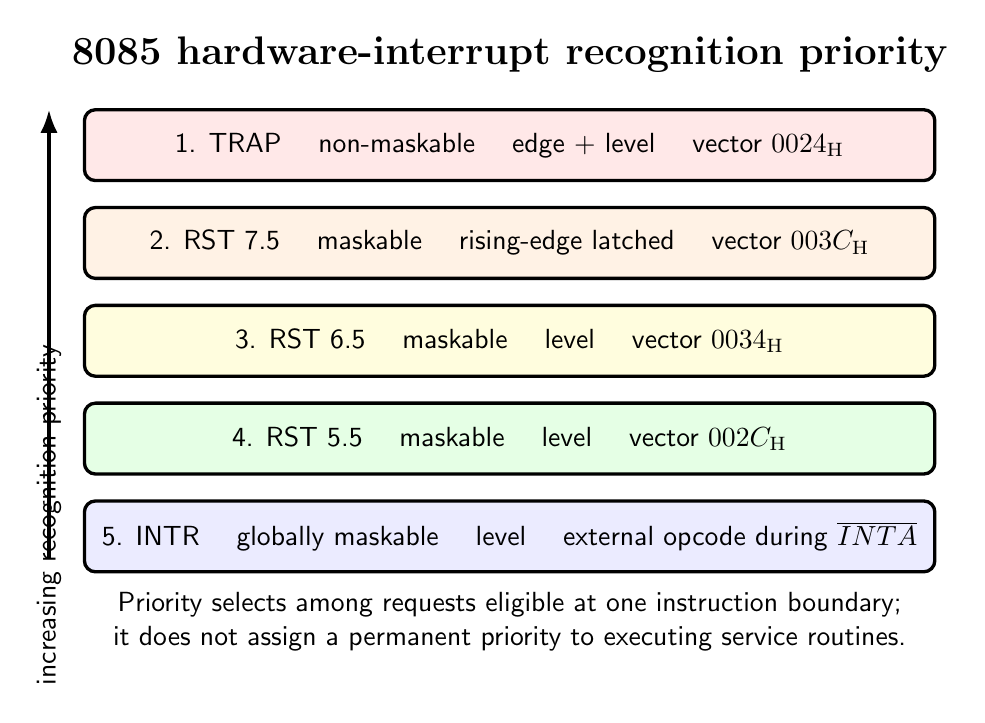
\begin{tikzpicture}[font=\sffamily,>=Latex,
  irq/.style={draw,very thick,rounded corners,minimum width=10.8cm,minimum height=.9cm,align=center}]
\node[font=\Large\bfseries] at (5.6,6.15) {8085 hardware-interrupt recognition priority};
\node[irq,fill=red!9]    (t) at (5.6,5.0) {1. TRAP \quad non-maskable \quad edge + level \quad vector $0024_{\rm H}$};
\node[irq,fill=orange!10,below=3mm of t] (r7) {2. RST 7.5 \quad maskable \quad rising-edge latched \quad vector $003C_{\rm H}$};
\node[irq,fill=yellow!13,below=3mm of r7] (r6) {3. RST 6.5 \quad maskable \quad level \quad vector $0034_{\rm H}$};
\node[irq,fill=green!10,below=3mm of r6] (r5) {4. RST 5.5 \quad maskable \quad level \quad vector $002C_{\rm H}$};
\node[irq,fill=blue!8,below=3mm of r5] (intr) {5. INTR \quad globally maskable \quad level \quad external opcode during $\overline{INTA}$};
\draw[very thick,->] (-.25,-.25)--(-.25,5.45) node[midway,left,rotate=90] {increasing recognition priority};
\node[align=center] at (5.6,-1.05) {Priority selects among requests eligible at one instruction boundary;\\it does not assign a permanent priority to executing service routines.};
\end{tikzpicture}
\end{document}
